\begin{figure}[H]
\centering
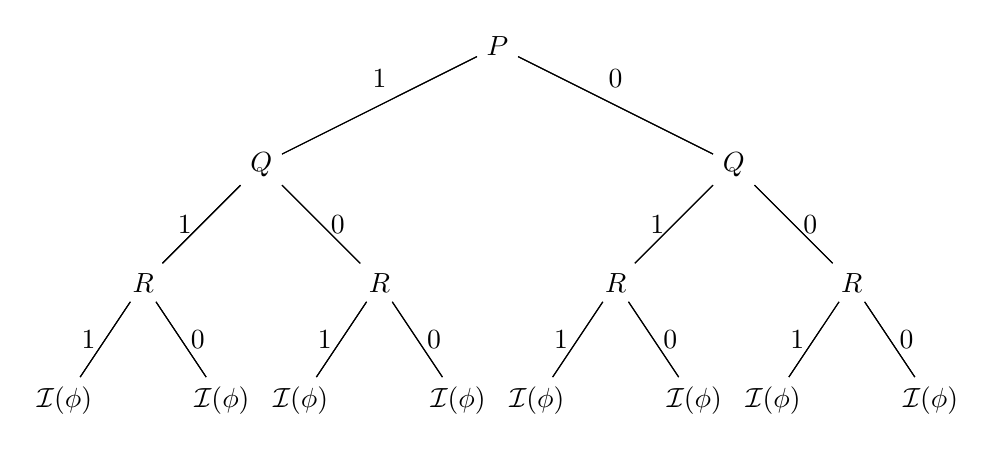
\begin{tikzpicture}[level/.style={sibling distance=60mm/#1}]
  \node (a) {$P$}
    child {node (b) {$Q$}
      child {node (d) {$R$}
      	child {node (dl) {$\mathcal{I}(\phi)$}}
      	child {node (dr) {$\mathcal{I}(\phi)$}}
      	}
      child {node (e) {$R$}
      	child {node (el) {$\mathcal{I}(\phi)$}}
      	child {node (er) {$\mathcal{I}(\phi)$}}
      	}
    }
    child {node (c) {$Q$}
    child {node (f) {$R$}
    	child {node (fl) {$\mathcal{I}(\phi)$}}
    	child {node (fr) {$\mathcal{I}(\phi)$}}
    	}
      child {node (g) {$R$}
      	child {node (gl) {$\mathcal{I}(\phi)$}}
      	child {node (gr) {$\mathcal{I}(\phi)$}}
      	}
    }; 	
%\path (a) -- (b) node {TRUE};
\path (a) edge node[above=3pt]{$1$} (b);
\path (a) edge node[above=3pt]{$0$} (c);

\path (b) edge node[left]{$1$} (d);
\path (b) edge node[right]{$0$} (e);
\path (c) edge node[left]{$1$} (f);
\path (c) edge node[right]{$0$} (g);

\path (d) edge node[left]{$1$} (dl);
\path (d) edge node[right]{$0$} (dr);
\path (e) edge node[left]{$1$} (el);
\path (e) edge node[right]{$0$} (er);
\path (f) edge node[left]{$1$} (fl);
\path (f) edge node[right]{$0$} (fr);
\path (g) edge node[left]{$1$} (gl);
\path (g) edge node[right]{$0$} (gr);
\end{tikzpicture}
\caption{Árbol de asignaciones de valores con tres variables.} \label{fig:a3sat01}
\end{figure}